\documentclass[10pt,twocolumn,a4paper]{article}
\usepackage[T1]{fontenc}
\usepackage[utf8]{inputenc}
\usepackage{polski,lmodern}
\usepackage[margin=18mm,columnsep=7mm]{geometry}
\usepackage{microtype,graphicx}
\usepackage{booktabs,tabularx,array}
\usepackage{amsmath,amssymb}
\usepackage{enumitem,placeins,xcolor,xurl,float,needspace,etoolbox}
\usepackage[hidelinks,breaklinks=true]{hyperref}
\hypersetup{pdftitle={Przewidywanie wskaźnika C/Z spółek giełdowych}}
\setlist[itemize]{leftmargin=*,itemsep=1pt,topsep=3pt}
\setlength{\emergencystretch}{1em}
\usepackage{balance}
\raggedbottom
\setlength{\textfloatsep}{8pt plus 2pt minus 2pt}
\setlength{\floatsep}{6pt plus 2pt minus 2pt}
\setlength{\intextsep}{6pt plus 2pt minus 2pt}
\pretocmd{\section}{\Needspace{6\baselineskip}}{}{}
\pretocmd{\subsection}{\Needspace{5\baselineskip}}{}{}
\newcolumntype{Y}{>{\raggedright\arraybackslash}X}
\renewcommand{\abstractname}{Streszczenie}

\newcommand{\TematProjektu}{Przewidywanie wskaźnika C/Z spółek giełdowych}
\newcommand{\TypZadania}{regresja}

\title{\TematProjektu\\[2mm]
\large Zaawansowane metody uczenia maszynowego}
\author{Szymon Poznański\\\small Numer albumu 146988
\and Hubert Chruścicki\\\small Numer albumu 146932}
\date{\quad \today}

\begin{document}
\maketitle

\begin{abstract}
Celem projektu jest sprawdzenie, czy da się przewidzieć wskaźnik cena/zysk, w skrócie C/Z, po angielsku P/E, spółki giełdowej na podstawie jej wskaźników finansowych z ostatnich czterech kwartałów. Przewidujemy nie sam C/Z, tylko jego logarytm, bo C/Z ma bardzo skośny rozkład, a kilka skrajnych spółek psułoby model. Dane pochodzą z zestawu \emph{Global Stock Market Dataset} z Kaggle. Po oczyszczeniu zostało 4\,677 spółek z wartością C/Z. Podział na zbiory jest grupowy, czyli kopie tej samej spółki zawsze trafiają do jednego zbioru, a proporcje to 70/15/15. Cały proces powtarzamy dla 20 losowych podziałów, żeby wynik nie zależał od jednego szczęśliwego losowania. Wybrany model to zwykła regresja liniowa na 13 cechach liczbowych i sektorze, a brakujące wartości uzupełniamy medianą. Na walidacji, po uśrednieniu 20 podziałów, model osiąga RMSE na skali logarytmicznej 0,94 $\pm$ 0,06, a prosty punkt odniesienia, czyli stała średnia, 1,15 $\pm$ 0,07. To poprawa o około 18\%. Na jednym podziale testowym, czyli seedzie 42, RMSE wynosi 0,950, a dla stałej średniej 1,164. Współczynnik R$^2$ to około 0,33, więc model tłumaczy mniej więcej jedną trzecią zmienności. Dane giełdowe są bardzo zaszumione, a nasze możliwości ograniczały braki i wartości skrajne. Wynik traktujemy jako uczciwy punkt odniesienia, a nie jako narzędzie inwestycyjne.
\end{abstract}

\section{Problem, motywacja i cel}
\subsection{Pytanie predykcyjne}
\textbf{Typ zadania:} \TypZadania{}, cel ciągły.

\noindent\textbf{Kontrakt predykcji:}
jednostką obserwacji jest spółka giełdowa w jednym momencie. Dane to jedna migawka, więc nie ma w nich osi czasu. Przewidujemy $\log(\text{C/Z})$, czyli logarytm kolumny \texttt{price\_earnings\_ttm}. Jako cechy bierzemy wskaźniki rentowności, płynności i zadłużenia, wielkość firmy w postaci logarytmów przychodów i aktywów oraz sektor. Zakładamy, że wszystkie te informacje są znane w chwili wyceny. Zastosowanie jest takie: model ma dać wstępną ocenę, czy C/Z spółki zgadza się z jej wskaźnikami finansowymi. Odbiorcą jest osoba, która jest ciekawa, czy w ogóle da się jakoś przewidzieć potencjał spółki na podstawie jej wskaźników fundamentalnych. Model nie jest narzędziem inwestycyjnym i nie służy do podejmowania decyzji o kupnie akcji.

\subsection{Kryterium użyteczności}
Najprostszy sposób przewidywania C/Z to dawać każdej spółce taką samą wartość, czyli średnią $\log(\text{C/Z})$ z treningu. Taki baseline w ogóle nie patrzy na wskaźniki finansowe, a na zbiorze testowym ma RMSE 1,164. Model ma sens tylko wtedy, gdy wyraźnie go pokona, bo to znaczy, że wskaźniki fundamentalne rzeczywiście coś mówią o wycenie spółki. Za wyraźną poprawę uznajemy niższe RMSE nie tylko na jednym podziale, ale konsekwentnie w większości z 20 losowych podziałów. Pytanie, na które odpowiadamy, nie dotyczy więc tego, czy model trafia w C/Z co do jednostki, tylko tego, ile da się wyjaśnić samymi fundamentami w porównaniu z brakiem jakiejkolwiek wiedzy.

\section{Dane i analiza wstępna}
\subsection{Źródło i znaczenie kolumn}
Dane pochodzą z zestawu \emph{Global Stock Market Dataset}, którego autorem jest Mehdi Aminazadeh. Źródło to \url{https://www.kaggle.com/datasets/mehdiaminazadeh/global-stock-market-dataset}. Pobieramy je przez bibliotekę \texttt{kagglehub}. Zestaw składa się z siedmiu plików CSV. Za bazę przyjęliśmy plik \texttt{tradingview\_all\_stocks}, bo tylko on zawiera zmienną, którą przewidujemy, a pozostałe pliki dołączamy do niego po kolumnie \texttt{ticker}. Plik bazowy ma 11\,806 wierszy i 10 kolumn. Po połączeniu wszystkich plików mamy 36 kolumn, a po dodaniu wskaźników pochodnych 45. Do modelu wybraliśmy 16 kolumn: 13 cech liczbowych, sektor, ticker i cel. Po odrzuceniu spółek bez C/Z i tych z C/Z poniżej 0,1 zostaje 4\,677 spółek. Znaczenie kolumn użytych w modelu opisuje Tabela \ref{tab:dane}.

\begin{table}[H]
\centering
\caption{Słownik danych używanych w modelu.}
\label{tab:dane}
\scriptsize
\setlength{\tabcolsep}{3pt}
\renewcommand{\arraystretch}{0.95}
\begin{tabularx}{\columnwidth}{@{}l>{\raggedright\arraybackslash}Xl@{}}
\toprule
Kolumna & Znaczenie & Rola\\
\midrule
\texttt{price\_earnings\_ttm} & C/Z, cena/zysk z 12 mies. & cel, log\\
\texttt{net\_margin\_ttm} & marża netto & cecha\\
\texttt{operating\_margin\_ttm} & marża operacyjna & cecha\\
\texttt{roe} & zwrot z kapitału własnego & cecha\\
\texttt{roa} & zwrot z aktywów & cecha\\
\texttt{dividend\_payout\_ratio\_ttm} & udział dywidendy w zysku & cecha\\
\texttt{current\_ratio\_fq} & płynność bieżąca & cecha, braki\\
\texttt{quick\_ratio\_fq} & płynność szybka & cecha, braki\\
\texttt{cash\_ratio} & płynność gotówkowa & cecha, braki\\
\texttt{debt\_to\_equity\_fq} & dług do kapitału własnego & cecha\\
\texttt{net\_debt\_to\_assets} & dług netto do aktywów & cecha\\
\texttt{liab\_to\_assets} & zobowiązania do aktywów & cecha\\
\texttt{slog\_revenue} & logarytm przychodów & cecha\\
\texttt{slog\_assets} & logarytm aktywów & cecha\\
\texttt{sector} & branża, 20 kategorii & one-hot\\
\bottomrule
\end{tabularx}
\end{table}

\subsection{Przygotowanie danych: co usunięto}
Dane przechodzą przez kilka etapów i na każdym odpada część spółek albo kolumn. Tabela \ref{tab:etapy} pokazuje, ile spółek zostaje po każdym z nich.

\begin{table}[!ht]
\centering
\caption{Liczba spółek na kolejnych etapach przygotowania danych.}
\label{tab:etapy}
\footnotesize
\begin{tabularx}{\columnwidth}{@{}Yr@{}}
\toprule
Etap & Spółki\\
\midrule
plik bazowy, \texttt{tradingview\_all\_stocks} & 11\,806\\
po usunięciu powtórek tickerów, 131 wierszy & 11\,675\\
spółki z C/Z; bez C/Z 6\,978 & 4\,697\\
po usunięciu C/Z $<$ 0,1 & 4\,677\\
z kompletem 13 cech, complete-case & 3\,394\\
\bottomrule
\end{tabularx}
\end{table}

\textbf{Kto odpada.}
\begin{itemize}
\item Spółki bez C/Z. Źródło po prostu nie podaje dla nich wartości. Większość z nich, czyli 4\,706 spółek, ma ujemny zysk netto, więc C/Z nie ma dla nich sensu.
\item Spółki z C/Z poniżej 0,1, czyli 20 przypadków. Takie C/Z oznaczałoby, że cena akcji jest mniejsza niż jedna dziesiąta rocznego zysku na akcję, co wygląda na błąd jednostek. To tylko nasza hipoteza i nie mamy pewności. Jest to jedyny przypadek, w którym wycinamy wartości odstające.
\item Spółki z brakami w cechach. Przy podejściu complete-case odpada 1\,283 z 4\,677 spółek, czyli 27\%. Dlatego w modelu używamy imputacji, którą opisujemy w sekcji 5.
\item Powtórki tickerów. Ta sama spółka występuje w kilku wierszach, więc zostawiamy tylko pierwszy z nich.
\end{itemize}

\textbf{Kolumny.} Z 45 kolumn zostawiamy 16. Odrzuciliśmy kilka grup kolumn. Po pierwsze, te, które zdradzają wynik, na przykład kapitalizację rynkową, bo C/Z to właśnie kapitalizacja podzielona przez zysk. Po drugie, ruch kursu, czyli \texttt{change} i \texttt{Perf.*}. To stopy zwrotu, które mówią o nastrojach na rynku, a nie o wynikach firmy. Po trzecie, surowe kwoty, z których policzyliśmy już wskaźniki. Po czwarte, kolumny z ponad 40\% braków, czyli marże brutto, EBITDA i FCF. Próg 40\% leży w największej przerwie między odsetkami braków: ostatnia zostawiona cecha miała 33,8\%, a pierwsza odrzucona 42,1\%. Po piąte, \texttt{industry}, które ma aż 130 kategorii, oraz \texttt{exchange}, bo giełda to miejsce notowania, a nie cecha firmy. W kolumnach ze zmianami kursu były też wartości zastępcze, na przykład 999\,900\%. Zamieniliśmy je na braki, w sumie 136 komórek. Dzielenie przez zero w naszych obliczeniach również dawało braki, w sumie 1\,834 wartości.

\subsection{Jakość i struktura danych}
Dane giełdowe są trudne z kilku powodów. Po pierwsze, sygnał jest słaby, bo C/Z zależy też od oczekiwań inwestorów i od kursu, a nie tylko od bieżących wskaźników firmy. Po drugie, sam cel jest zaszumiony: gdy zysk spółki jest bliski zera, jej C/Z robi się ogromne. Dlatego logarytmujemy cel i usuwamy oczywiste błędy jednostek, czyli C/Z poniżej 0,1. Po trzecie, braki występują we wszystkich 13 cechach, od 14,6\% do 33,8\%, i są rozłożone nierówno. Sektor Finance to 30,8\% zbioru treningowego, ale aż 93,8\% spółek z brakiem płynności. Po czwarte, wiele spółek to kopie tej samej firmy. Na przykład GOOG i GOOGL mają identyczne cechy, więc podział na zbiory musi być grupowy. Wartości podejrzane zostawiamy w danych, bo nie mamy dowodu, że są błędne. Na przykład w 35 przypadkach $|$ROA$|$ jest większe niż 100\%, czyli zwrot z aktywów wynosi ponad 100\% albo poniżej $-100\%$.

\textbf{Braki.} Braki nie są błędem, który sami wprowadziliśmy. Wynikają z natury danych, bo źródło nie podaje wartości dla części spółek. C/Z brakuje u 6\,978 spółek, czyli 59,8\%, głównie takich ze stratą. Z nich 4\,706 ma ujemny zysk netto, więc wskaźnik nie ma sensu, a źródło zostawia pole puste. Dodatkowo 204 spółki z dodatnim zyskiem również nie mają C/Z. Wskaźniki pochodne są puste, gdy mianownik jest zerem albo go brakuje. Wartości z dzielenia przez zero, w sumie 1\,834, zamieniliśmy na braki.

Co z tymi brakami zrobiliśmy? Spółki bez C/Z odpadają, bo cel jest wymagany i nie uzupełniamy go. Braki w 13 cechach uzupełniamy imputacją, którą opisujemy w sekcji 5, a podejście complete-case zostaje punktem odniesienia. Warto pamiętać, że braki nie są losowe. Mediana C/Z spółek kompletnych to 20,9, a spółek z brakami 11,7. Complete-case jest więc przesunięty w stronę spółek o wyższym C/Z.

\textbf{Wartości odstające.} Na box-plotach wiele cech ma 10-25\% wartości poza wąsami. Surowe kwoty, czyli aktywa, przychody i kapitalizacja, leżą nisko, a pojedyncze kropki sięgają bardzo wysoko. Po zlogarytmowaniu większość pudełek mieści się w rozsądnym zakresie. Zysk netto, wolny przepływ gotówki i EBITDA mają po logarytmie dwa garby, bo rozdzielają spółki na zyskowne i stratne. Kilka cech, na przykład dług i dywidenda, ma słupek dokładnie przy zerze, bo część spółek ich po prostu nie ma. Wartości odstające traktujemy jako część rozkładu, a nie błąd, więc nie usuwamy ich. Wyjątkiem jest C/Z poniżej 0,1.

\textbf{Rozkład celu.} C/Z ma medianę 18, średnią 86,2 i odchylenie standardowe 1\,312. To wskaźnik bezwymiarowy: pokazuje, ile razy cena akcji jest większa od rocznego zysku na akcję. Skośność wynosi 44,6, a po zlogarytmowaniu 1,0. Dlatego model przewiduje $\log(\text{C/Z})$.

\textbf{Kontrola danych błędnych.} Na zbiorze, który trafia do modelu, wykonaliśmy sześć sprawdzeń i każde dało wynik 0. Sprawdzaliśmy powtórki tickerów, nieskończoności, C/Z $\le$ 0, \texttt{cash\_ratio} poza przedziałem $[0,1]$, ujemne wskaźniki płynności i zadłużenia oraz braki po imputacji. Wartości podejrzane zostawiliśmy. 164 spółki mają \texttt{liab\_to\_assets} większe niż 1, czyli ujemny kapitał własny, co jest możliwe z punktu widzenia księgowości. 35 spółek ma $|$ROA$|$ większe niż 1. 6 spółek ma marżę powyżej 10\,000\%, bo ich przychód jest bliski zeru. Dwie wartości powyżej 100\,000 to pojedyncze komórki w kolumnach \texttt{net\_margin\_ttm} i \texttt{roe}.

\subsection{Najważniejsze obserwacje z EDA}
\begin{figure}[t]
\centering
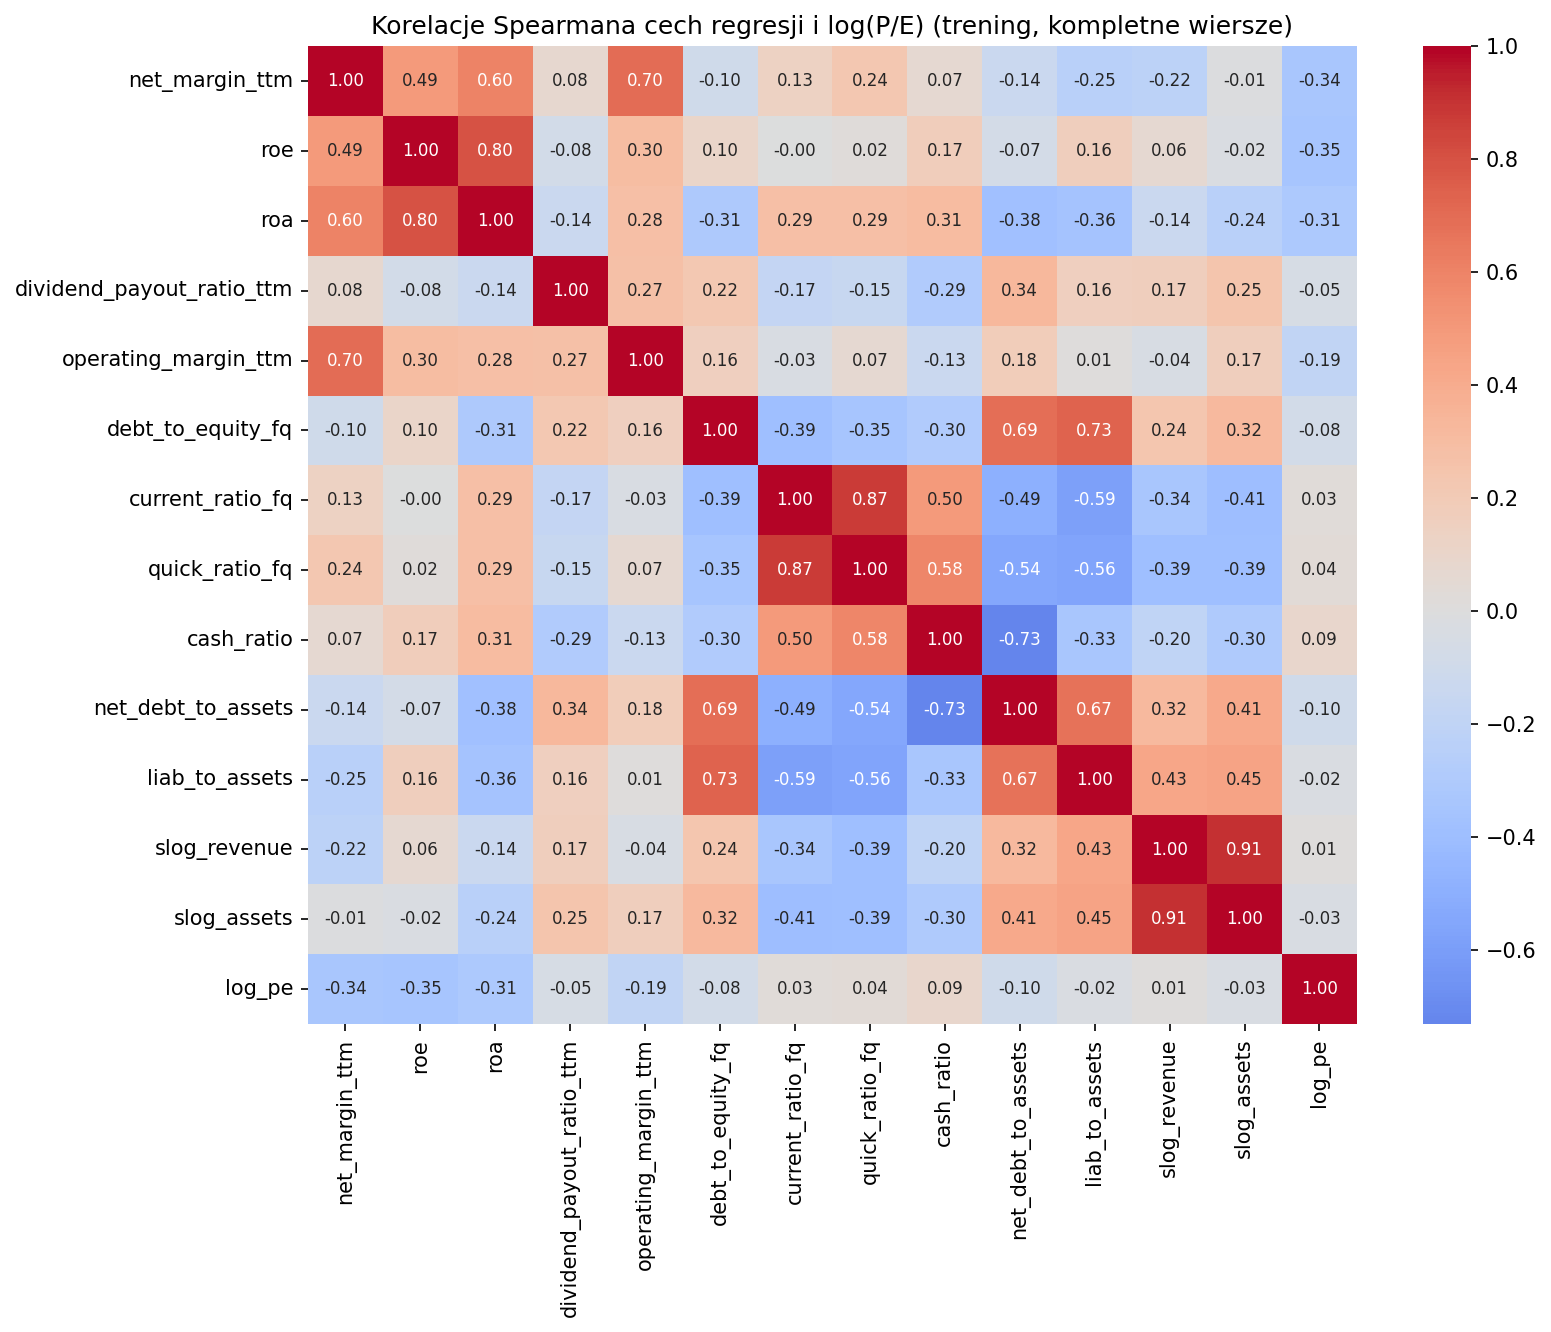
\includegraphics[width=0.85\columnwidth]{rysunki/fig_korelacje_nb.png}
\caption{Korelacje Spearmana cech i log(C/Z) na zbiorze treningowym.}
\label{fig:korelacje}
\end{figure}

\begin{figure*}[t]
\centering
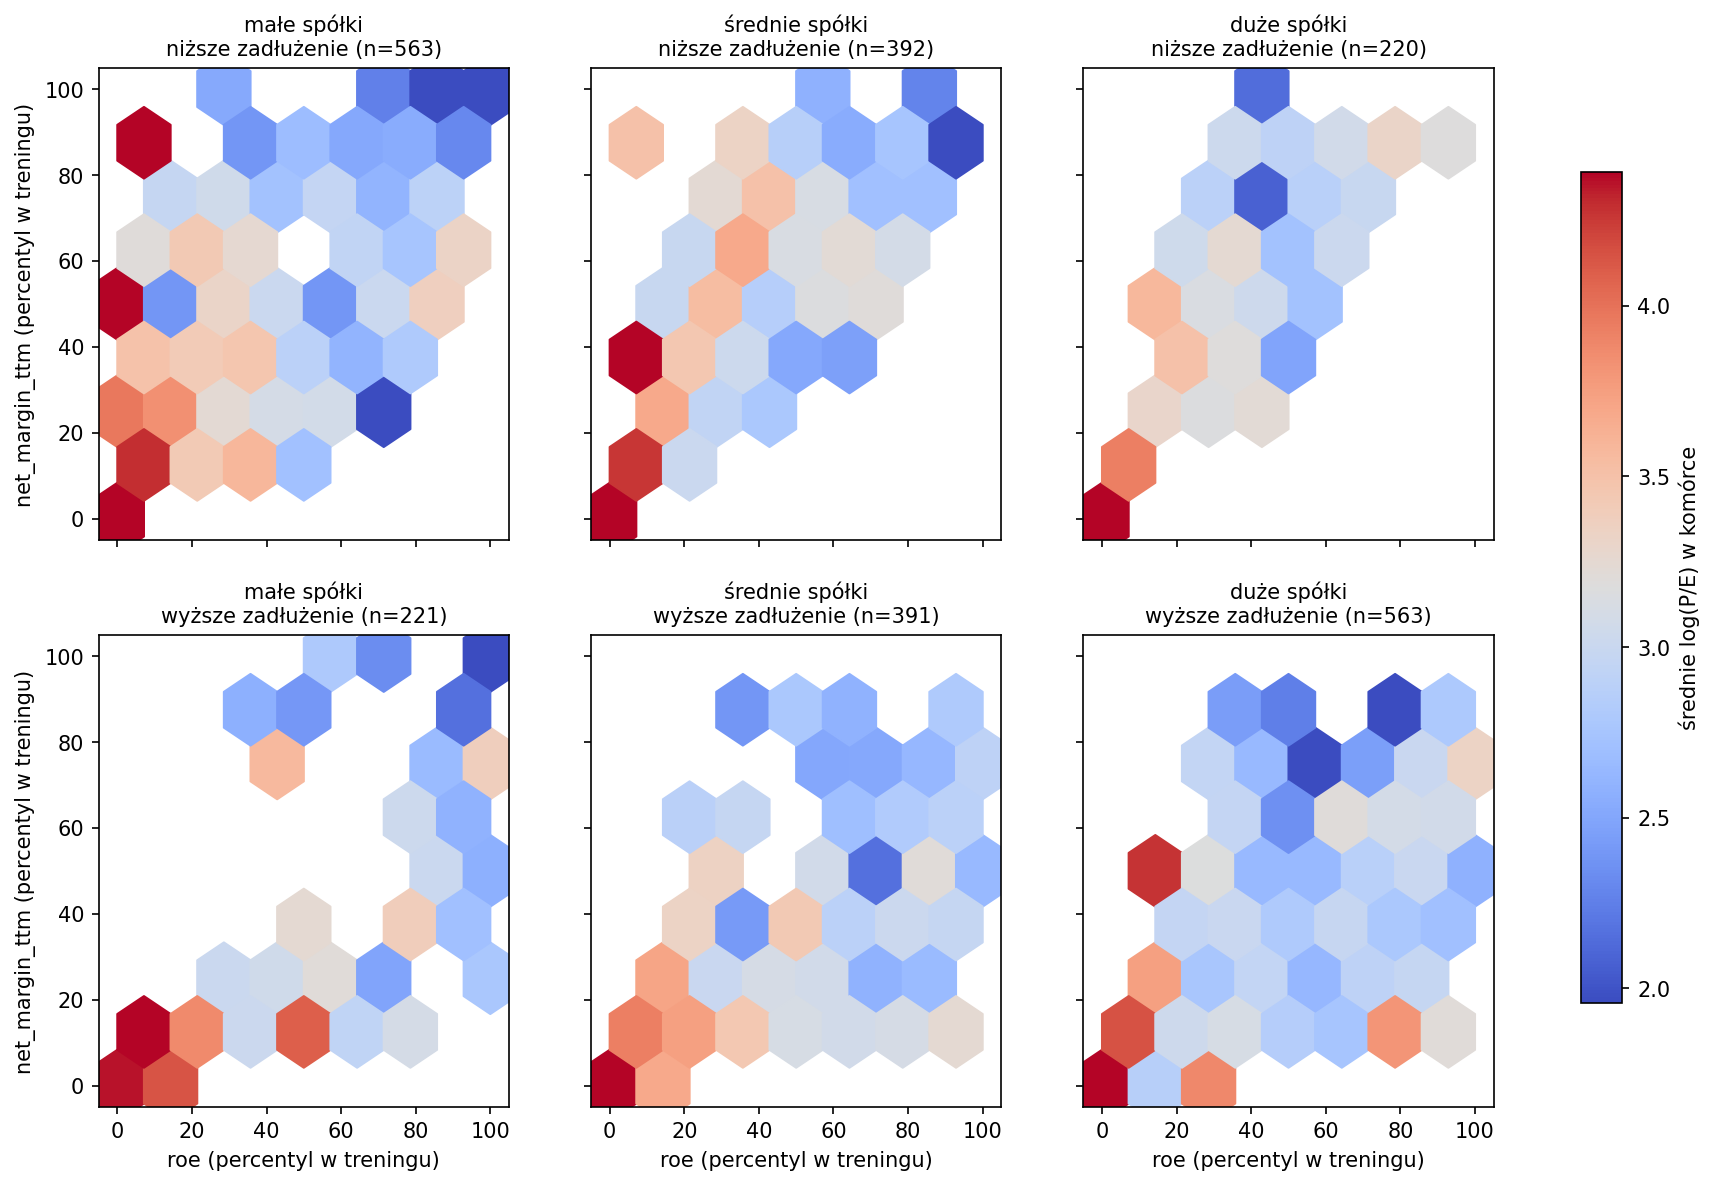
\includegraphics[width=0.8\textwidth]{rysunki/fig_piec_zmiennych_nb.png}
\caption{Średni log(C/Z) w komórkach. ROE i marża netto w percentylach treningu. Osobno dla wielkości spółki, w kolumnach, i zadłużenia, w wierszach. Kolor oznacza średni log(C/Z) w komórce.}
\label{fig:piec}
\end{figure*}

\begin{figure}[t]
\centering
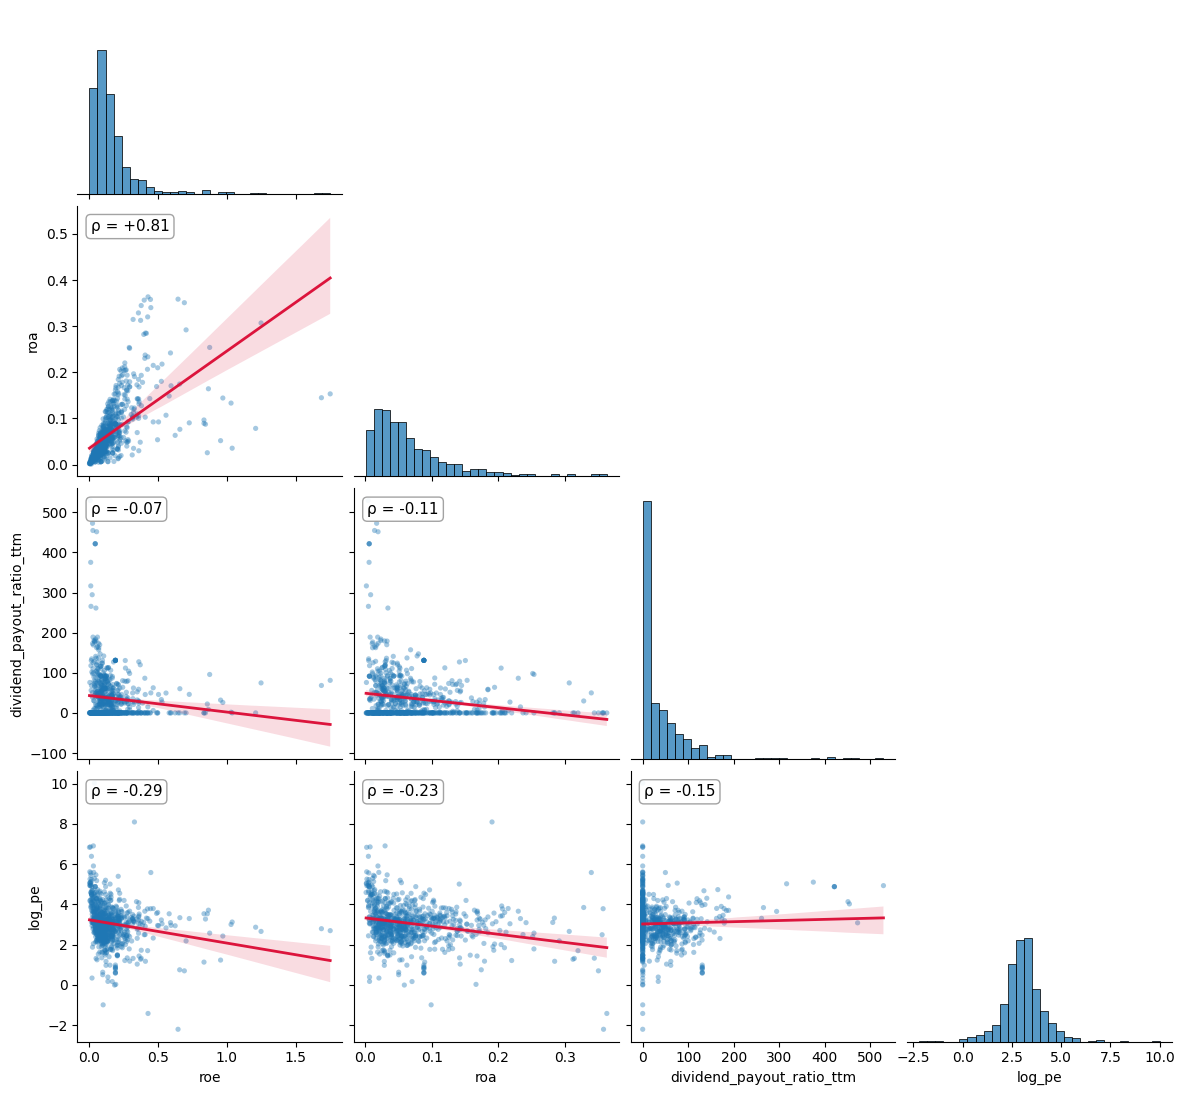
\includegraphics[width=\columnwidth]{rysunki/fig_pairplot_zwrot_nb.png}
\caption{Wykresy rozrzutu ROE, ROA, wypłaty dywidendy i log(C/Z) dla próbki 800 spółek z treningu. Na przekątnej histogramy, w ramce korelacja Spearmana, czerwona linia to trend liniowy.}
\label{fig:pairplot}
\end{figure}

Po zlogarytmowaniu skośność C/Z spada z 44,6 do około 1, więc logarytm to dobry wybór celu.

Rys. \ref{fig:korelacje} pokazuje korelacje Spearmana policzone na zbiorze treningowym, czyli na 2\,350 spółkach z kompletem cech. Cechy rentowności mają umiarkowany, ujemny związek z log(C/Z). Dla ROE korelacja wynosi $\rho = -0{,}35$, dla marży netto $-0{,}34$, a dla ROA $-0{,}31$. To ma sens, bo zysk stoi w mianowniku C/Z. Wskaźniki zadłużenia są prawie niezwiązane z C/Z.

\textbf{Współliniowość.} Sześć par cech ma $|\rho| > 0{,}7$, czyli w każdej z nich jedna cecha niesie prawie tę samą informację co druga:
\begin{itemize}
\item przychody i aktywa: $0{,}91$,
\item płynność bieżąca i szybka: $0{,}87$,
\item ROE i ROA: $0{,}80$,
\item dług do kapitału i zobowiązania do aktywów: $0{,}73$,
\item gotówka i dług netto: $-0{,}73$,
\item marża netto i operacyjna: $0{,}70$.
\end{itemize}
Mimo to zostawiamy wszystkie 13 cech. Wariant z 9 cechami dawał więcej kompletnych wierszy, 4\,165 zamiast 3\,394, ale nadal zostawiał nierozwiązane pary ROE i ROA oraz zadłużenia. Współczynniki pojedynczych cech z takich par są niestabilne, więc nie interpretujemy ich osobno. Jeszcze jedna uwaga: \texttt{debt\_to\_equity\_fq} ma tylko 30 różnych wartości, i to całkowitych, czyli źródło je zaokrągla. Wszystko, co tu opisujemy, to obserwacje korelacyjne, a nie dowód przyczynowości.

Rys. \ref{fig:piec} pokazuje, że średni log(C/Z) maleje wraz z ROE i marżą. Ten wzór powtarza się we wszystkich sześciu panelach, więc wielkość spółki i jej zadłużenie nie przesuwają poziomu C/Z. Mediany w panelach mieszczą się w przedziale 18,6-22,3, a dla wszystkich spółek wynoszą 20,7. Zmienia się natomiast siła związku. Dla ROE korelacja wynosi $-0{,}48$ dla małych spółek o niższym zadłużeniu i $-0{,}19$ dla dużych o niższym zadłużeniu. Spółki z dolnych 25\% obu cech, czyli 343 spółki, mają medianę C/Z równą 50,2. Spółki z górnych 25\%, czyli 256, mają 13,7. Wielkość i zadłużenie są ze sobą powiązane, bo wyższe zadłużenie ma 72\% dużych spółek, a małych tylko 28\%. Dlatego z wykresu nie da się rozdzielić ich wpływów.

Rys. \ref{fig:pairplot} pokazuje te same zależności na pojedynczych spółkach, dla ROE, ROA i wypłaty dywidendy. To próbka 800 spółek z treningu, a osie przycięliśmy do 1-99 percentyla tylko po to, żeby wykres był czytelny. Dane w analizie zostały bez zmian. ROE i ROA rosną razem, bo $\rho = 0{,}81$ w próbce, co potwierdza współliniowość tej pary. Wobec log(C/Z) ROE ma $\rho = -0{,}29$, ROA $-0{,}23$, a wypłata dywidendy $-0{,}15$. Czerwona linia dla wypłaty dywidendy idzie lekko w górę mimo ujemnej korelacji, bo ciągnie ją 67 spółek z wypłatą powyżej 200\%. Zysk bliski zera zawyża jednocześnie wypłatę dywidendy i C/Z, więc obie wartości mogą mieć jedną przyczynę. W prawym dolnym rogu widać rozkład celu: log(C/Z) jest dzwonowy, skupiony wokół 3, czyli C/Z około 20, z krótkim lewym ogonem do $-2$ i prawym do około 11.



\section{Protokół eksperymentu}
\subsection{Podział i granica dopasowania}
Podział na zbiory jest grupowy i zrobiliśmy go przy pomocy \texttt{GroupShuffleSplit}. Powód jest taki, że ta sama firma może występować w danych kilka razy, na przykład jako akcje zwykłe i uprzywilejowane. Gdyby jedna kopia trafiła do treningu, a druga do testu, model widziałby w treningu niemal tę samą spółkę, którą ma potem przewidzieć, i wynik byłby zawyżony. Wiersze o identycznym wektorze 13 cech uznajemy więc za jedną grupę i zawsze trafiają one do jednego zbioru.

To przybliżenie, bo dwie różne firmy o identycznych cechach też trafią do jednej grupy. Jest to jednak bezpieczniejszy błąd, bo nie zawyża wyniku, choć nie jest dokładną identyfikacją firmy. Sprawdziliśmy, że 366 z 3\,402 wierszy complete-case, czyli 10,8\%, ma taki sam wektor cech jak jakiś inny wiersz. Daje to 130 grup, na przykład \texttt{NYSE:F} i \texttt{NYSE:F/PB}. W 75 z tych 130 grup kopie trafiłyby przy zwykłym losowym podziale do różnych zbiorów.

Liczebności zbiorów to 3\,288, 687 i 702 spółki. Proporcje są w przybliżeniu 70/15/15, dokładnie 70,3\%, 14,7\% i 15,0\%, bo dzielimy grupy, a nie pojedyncze wiersze. Wszystkie decyzje, czyli wybór imputacji, skalowania, kodowania i metody, podejmujemy na treningu i walidacji. Nie używamy walidacji krzyżowej. Mamy jeden podział na trening, walidację i test, który powtarzamy dla 20 seedów. Zbiór testowy oceniamy tylko jeden raz, na zamrożonej już procedurze.

Wynik zależy od tego, jak wylosował się podział, więc powtarzamy cały proces dla 20 ziaren losowości: seed 42 oraz seedy od 0 do 18. Seed 42 to podział bazowy z sekcji 4d notatnika. Każdy seed daje inny podział grupowy, który ustawiamy przez \texttt{random\_state}, więc indeksy da się odtworzyć. Imputację, one-hot, skalowanie i model dopasowujemy zawsze wyłącznie na treningu danego seeda. Walidacja ma w różnych seedach od 680 do 721 spółek. Raportujemy średnią i odchylenie z 20 seedów. Podziały nie są niezależne, bo każdy z nich losuje 15\% tych samych spółek. Odchylenie pokazuje więc, jak bardzo wynik zależy od losowania, ale nie jest błędem standardowym w sensie statystycznym.

\subsection{Metryka główna i miary pomocnicze}
\noindent\textbf{Miara główna:} RMSE na skali $\log(\text{C/Z})$. Im jest niższe, tym lepiej. Wybraliśmy je dlatego, że przy błędzie liczonym wprost na C/Z wynik zdominowałyby spółki o bardzo wysokim wskaźniku, rzędu tysięcy. RMSE na logu ma jednostki celu i pokazuje błąd względny. Błąd 0,3 w logu to około 35\% różnicy w C/Z, niezależnie od tego, jak duże jest samo C/Z.

\noindent\textbf{Miary pomocnicze:} MAE na skali logarytmicznej, błąd procentowy $\exp(\text{MAE})-1$, czyli średni błąd C/Z w procentach, oraz MedAE w jednostkach C/Z, która jest odporna na skrajne wartości. Podajemy też R$^2$ na skali logarytmicznej. Wartość ujemna oznaczałaby model gorszy niż stała średnia.

\section{Preprocessing i baseline}
\begin{figure*}[t]
\centering
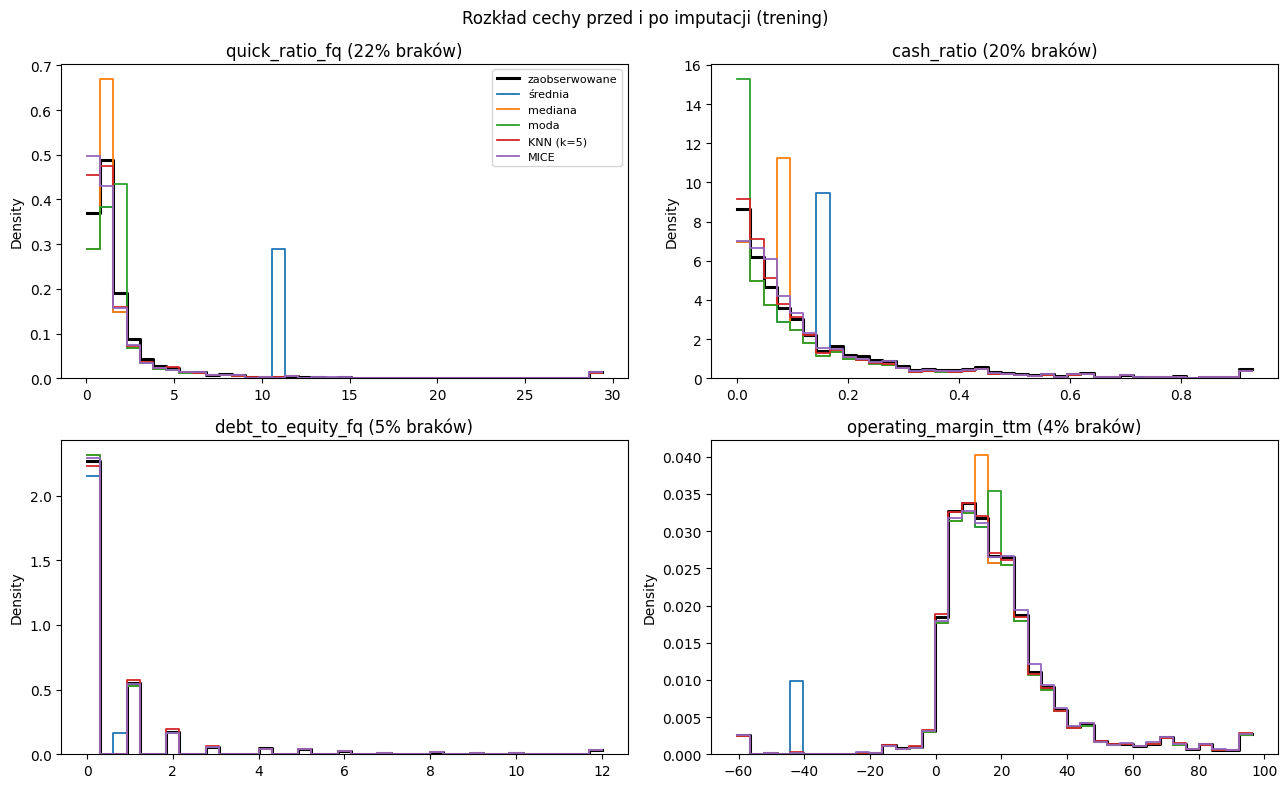
\includegraphics[width=0.8\textwidth]{rysunki/fig_imputacja_nb.png}
\caption{Rozkład czterech cech z największym odsetkiem braków przed i po imputacji, zbiór treningowy. Czarna linia to wartości zaobserwowane. Osie przycięte do 1-99 percentyla.}
\label{fig:imputacja}
\end{figure*}

\begin{figure}[t]
\centering
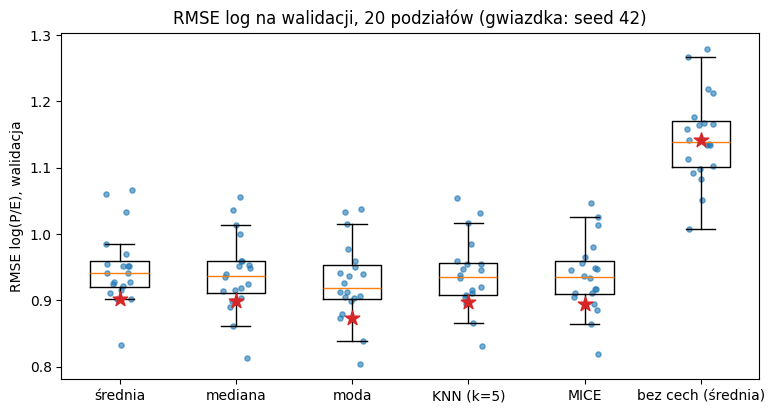
\includegraphics[width=\columnwidth]{rysunki/fig_seedy_nb.png}
\caption{RMSE na walidacji dla 20 podziałów, pięciu metod imputacji i modelu bez cech. Gwiazdka oznacza seed 42.}
\label{fig:seedy}
\end{figure}

\textbf{Dlaczego preprocessing jest trudny.} Każde przekształcenie to jakiś kompromis. Logarytmujemy cel, żeby ogony nie dominowały. Uzupełniamy braki zamiast usuwać spółki, bo usunięcie dotknęłoby głównie firm finansowych. Używamy skalowania rangowego zamiast zwykłej standaryzacji, która dawała RMSE około 10,7-11,2, bo skrajne wartości psuły skalę. Odrzucamy część z 45 kolumn i używamy prostego modelu bez strojenia.

\textbf{Imputacja.} Braki uzupełniamy w potoku, który dopasowujemy na treningu. Porównujemy pięć metod: średnią, medianę, modę, KNN z 5 sąsiadami oraz MICE, czyli uzupełnianie regresją. Tabela \ref{tab:walidacja} podaje RMSE na walidacji dla 20 podziałów. Wszystkie metody są wyraźnie lepsze od stałej średniej, a różnice między nimi są małe. Najniższe średnie RMSE ma moda, ale mediana też była lepsza od stałej średniej we wszystkich 20 podziałach.

Wybieramy medianę, bo jest prostsza i odporniejsza na skrajne wartości. Uczciwie trzeba przyznać, że moda jest średnio lepsza o 0,012, więc to decyzja o prostocie, a nie o najlepszym wyniku. Przewaga mody jest systematyczna, bo jest lepsza od mediany w 16 z 20 seedów i najlepsza ze wszystkich w 14. Mimo to różnica między metodami w tym samym seedzie jest mniejsza niż rozrzut między seedami. Odchylenie różnicy między medianą a najlepszą metodą wynosi 0,007-0,014, a mediana nigdy nie traci do najlepszej więcej niż 0,024. Przyjęty przez nas próg remisu 0,03 jest więc większy od tego szumu. KNN i MICE praktycznie nie różnią się od mediany, bo różnica wynosi $-0{,}001$ i $-0{,}003$. Średnia jest najsłabsza, bo wypada średnio o 0,009 gorzej niż mediana.

Warto też wiedzieć, że braki płynności są strukturalne. Sektor Finance to 31\% treningu, ale aż 94\% spółek z brakiem \texttt{quick\_ratio\_fq} lub \texttt{cash\_ratio}, czyli 666 z 710. Banki i podobne firmy nie mają sensownych wskaźników płynności, więc imputacja wpisuje im wartość umowną, a nie pomiar. Informację o tym, że to firma finansowa, niesie za to sektor.

Rys. \ref{fig:imputacja} pokazuje, jak poszczególne metody zmieniają rozkład czterech cech z największym odsetkiem braków. Czarna linia to wartości zaobserwowane. Średnia tworzy osobny słupek daleko od głównej masy, na przykład dla \texttt{quick\_ratio\_fq} około 11 przy medianie 1,2, bo skrajne spółki ciągną ją w górę. Mediana i moda wpisują wszystkim jedną typową wartość, przez co rozkład się zagęszcza i jego rozrzut maleje. KNN i MICE najlepiej zachowują kształt rozkładu, choć też trochę go zwężają. To ocena kształtu rozkładów, a nie dokładności uzupełnień.

Rys. \ref{fig:seedy} pokazuje RMSE na walidacji dla każdego z 20 podziałów. Każdy punkt to jeden podział, gwiazdka to seed 42, a pudełko pokazuje rozrzut. Wszystkie metody imputacji mieszczą się w podobnym przedziale, od około 0,8 do 1,07, a model bez cech jest wyraźnie wyżej. Seed 42 leży w dolnej części rozrzutu, czyli był łaskawszy niż przeciętny podział.

\begin{table}[H]
\centering
\caption{RMSE na skali log(C/Z), walidacja, 20 podziałów: średnia i odchylenie.}
\label{tab:walidacja}
\footnotesize
\begin{tabularx}{\columnwidth}{@{}lYY@{}}
\toprule
Wersja & RMSE (średnia) & RMSE (odch.)\\
\midrule
braki uzupełnione średnią & 0,949 & 0,055\\
braki uzupełnione medianą, wybrana & 0,940 & 0,057\\
braki uzupełnione modą & 0,928 & 0,059\\
braki uzupełnione KNN, 5 sąsiadów & 0,939 & 0,054\\
braki uzupełnione MICE, regresja & 0,936 & 0,054\\
bez modelu: stała średnia & 1,145 & 0,067\\
\bottomrule
\end{tabularx}
\end{table}

\textbf{Complete-case a imputacja.} Podejście complete-case, czyli usunięcie spółek z brakami, traktujemy jako punkt odniesienia. Na tych samych 511 kompletnych spółkach walidacji wypada ono lepiej niż mediana z imputacją. RMSE wynosi 0,892 wobec 0,914, po uśrednieniu 20 podziałów, a complete-case wygrywa w 19 z 20 podziałów. Imputacja pozwala jednak ocenić wszystkie 687 spółek walidacji, także 176 z brakami. Na całej walidacji mediana ma RMSE 0,940, po uśrednieniu 20 podziałów, a na samych 511 kompletnych spółkach 0,914. Spółki z brakami są więc przewidywane nieco gorzej, ale model obejmuje dzięki temu znacznie więcej spółek. Dlatego to właśnie mediana trafia do modelu.

\textbf{Kolejność.} Najpierw robimy imputację medianą dopasowaną na treningu, potem one-hot sektora z kategoriami wziętymi z treningu, następnie skalę rang na cechach liczbowych, dopasowaną na treningu już po imputacji, a na końcu regresję. Każdy etap dopasowujemy tylko na treningu, a walidację i test jedynie przekształcamy.

\textbf{Skalowanie i kodowanie.} Cechy liczbowe skalujemy skalą rang, czyli klasą \texttt{RankScaler}. Każda wartość zostaje zastąpiona jej pozycją w rozkładzie treningowym, przeliczoną na kwantyl rozkładu normalnego. Sektor kodujemy metodą one-hot z kategorią odniesienia Finance, co daje 19 kolumn. Razem mamy 32 kolumny wejściowe. Kolumny one-hot zostają jako 0 i 1 i nie są skalowane.

\textbf{Model i baseline.} Model to regresja liniowa, \texttt{LinearRegression}, bez strojenia. Jest celowo prosta, bo ma być punktem odniesienia. Baseline to stała średnia $\log(\text{C/Z})$ policzona na treningu. Krzywa uczenia na Rys. \ref{fig:lc} pokazuje, że RMSE spada z 0,959 przy 10\% treningu, czyli około 330 spółkach. Przy 25\% wynosi 0,919, przy 50\% 0,905, przy 75\% 0,902, a przy 100\%, czyli 3\,288 spółkach, 0,898. Od 50\% w górę poprawa to tylko około 0,007, więc ograniczeniem jest raczej prosty model liniowy niż liczba spółek. Odchylenie między seedami wynosi 0,027 przy 10\% treningu i poniżej 0,01 od 50\% w górę. Zbiory walidacyjny i testowy są przez cały czas takie same.

\begin{figure}[H]
\centering
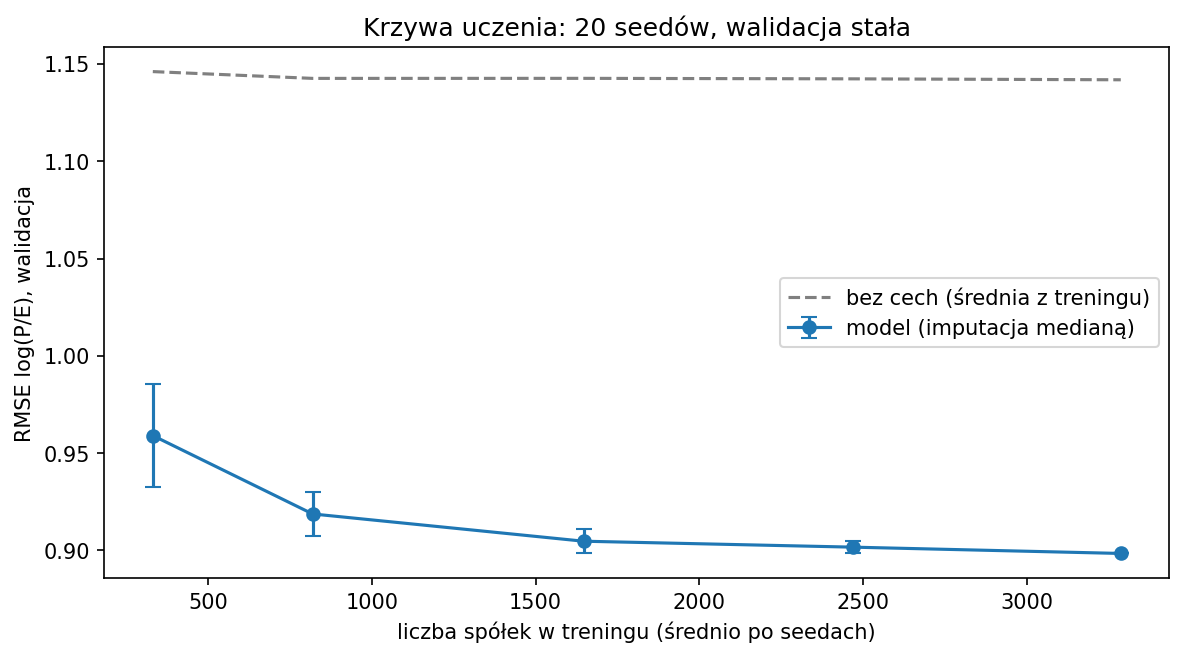
\includegraphics[width=0.85\columnwidth]{rysunki/fig_krzywa_uczenia_nb.png}
\caption{Krzywa uczenia: RMSE na walidacji w zależności od udziału treningu.}
\label{fig:lc}
\end{figure}

\balance
\textbf{Wynik testowy.} Tabela \ref{tab:test} porównuje wybrany model z baseline na tych samych 702 spółkach. Wersja bez uzupełniania braków, oceniana na 533 spółkach, wypada lepiej, ale mierzy inną grupę spółek, więc nie można jej wprost porównywać. Model jest o około 18\% lepszy od baseline. Jego błąd procentowy, równy 90\%, pokazuje, jak niepewne są pojedyncze wyceny.

Trzeba jednak pamiętać, że ta liczba pochodzi z jednego podziału, czyli seeda 42, który był łaskawszy niż przeciętny. Na walidacji RMSE dla tego seeda wynosi 0,898, a średnio po 20 podziałach 0,94 $\pm$ 0,06. Test to jedna próba, więc uczciwiej jest czytać wynik jako 0,94 $\pm$ 0,06 niż jako dokładne 0,950.

\begin{table}[H]
\centering
\caption{Wyniki na zbiorze testowym, seed 42.}
\label{tab:test}
\footnotesize
\setlength{\tabcolsep}{3pt}
\begin{tabularx}{\columnwidth}{@{}lYYYY@{}}
\toprule
Wersja & RMSE & MAE & R$^2$ & MedAE C/Z\\
\midrule
bez braków, 533 kompletne & 0,831 & 0,605 & 0,349 & 8,81\\
mediana, 533 kompletne & 0,851 & 0,609 & 0,316 & 8,62\\
\textbf{mediana, wszystkie 702} & \textbf{0,950} & \textbf{0,642} & \textbf{0,328} & \textbf{7,07}\\
stała średnia, 702 & 1,164 & 0,794 & $-$0,008 & 9,80\\
\bottomrule
\end{tabularx}
\end{table}

\FloatBarrier
\end{document}
